\documentclass[xcolor={dvipsnames}]{beamer}

\usetheme{Malmoe}
\usecolortheme{seagull}
\usepackage[]{natbib}
\usepackage{textpos}
\usepackage{amsmath, amssymb, bm}
\usepackage{multirow}
\usepackage{framed}
\usepackage{schemata}
\setbeamertemplate{navigation symbols}{}
\usepackage[english]{babel}
\usepackage{animate}
\usepackage{graphics}
\usepackage{fontawesome}


\definecolor{lightblue}{rgb}{0.145,0.6666,1} % Defines the color used for content box headers
\definecolor{Red}{rgb}{0.9,0.15,0}
\definecolor{Blue}{RGB}{55,126,184}
\definecolor{Green}{RGB}{77,175,74}
\definecolor{White}{RGB}{255,255,255}
\definecolor{Lightgray}{rgb}{0.86,0.86,0.86}

\setbeamertemplate{footline}
{
	\leavevmode%
	\hbox{%
		\begin{beamercolorbox}[wd=.50\paperwidth,ht=2.25ex,dp=1ex,center]{author in head/foot}%
			\usebeamerfont{author in head/foot}\insertshortauthor%% \beamer@ifempty{\insertshortinstitute}{}{(\insertshortinstitute)}
		\end{beamercolorbox}%
%		\hskip2pt%
		\begin{beamercolorbox}[wd=.50\paperwidth,ht=2.25ex,dp=1ex,center]{title in head/foot}%
			\usebeamerfont{title in head/foot}\insertshorttitle~~~~~~~~~~~~~~~~~~~~~~~~~~\insertframenumber
		\end{beamercolorbox}%
	}%
	\vskip0pt%
}
\makeatother

\title[Latin America's epidemic of violence]{}

\subtitle{\large{\textsc{Latin America's epidemic of violence and its impact on longevity and other health outcomes}}\\$\,$\\}


\author[JM Aburto. ANU September 2018]
{
	\vspace{-0.5cm}
	\texorpdfstring{
		\begin{columns}
			\column{.9\linewidth}
			\centering
			\Large{Jos\'{e} Manuel Aburto}\\
			$\,$\\
			
\includegraphics[scale=0.2]{Figures/SDU_Logo.jpg}\\     
				\vspace{0.5cm}
						\includegraphics[scale=0.2]{Figures/MPIDR.PNG}     
		\end{columns}
	}
	{}
}

\date[]{ September 2018}

\beamertemplatenavigationsymbolsempty
\begin{document}


\begin{frame}[plain]
	\titlepage
\end{frame}
%%%%%%%%%%%%%%%%%%%%%%%%%%%%%%%%%%%%%%%%%%%%%%%%%%%%%%%%%%%%%%%%%%%%%%%%%
%%%%%%%%%%%%%%%%%%%%%%%%%%%%%%%%%%%%%%%%%%%%%%%%%%%%%%%%%%%%%%%%%%%%%%%%%


%%%%%%%%%%%%%%%%%%%%%%%%%%%%%%%%%%%%%%%%%%%%%%%%%%%%%%%%%%%%%%%%%%%%%%%%%
\begin{frame}
\Large{
		\begin{itemize}
		
		\item<1-> \textbf{Latin America} is the world's most \textbf{violent} region.
		
		\item<2-> This region has the \textbf{highest} homicide rate in the world (16.3 per 100,000).
		
        \item<3-> Central American countries $\longrightarrow$ \textbf{upsurge} in homicides in the new century.

        \item<4-> \textbf{In Mexico, rates doubled between 2007 and 2012} (9.3 $\longrightarrow$ 18.6).
		
		\end{itemize}
		
}

\end{frame}


\begin{frame}\frametitle{As a result}

\Large{
		\begin{itemize}
		    
		\item Male life expectancy \textbf{stagnated} in the first decade of the 2000's ($\backsim $72y)
		
				\end{itemize}
		
		\pause
				\begin{center}
		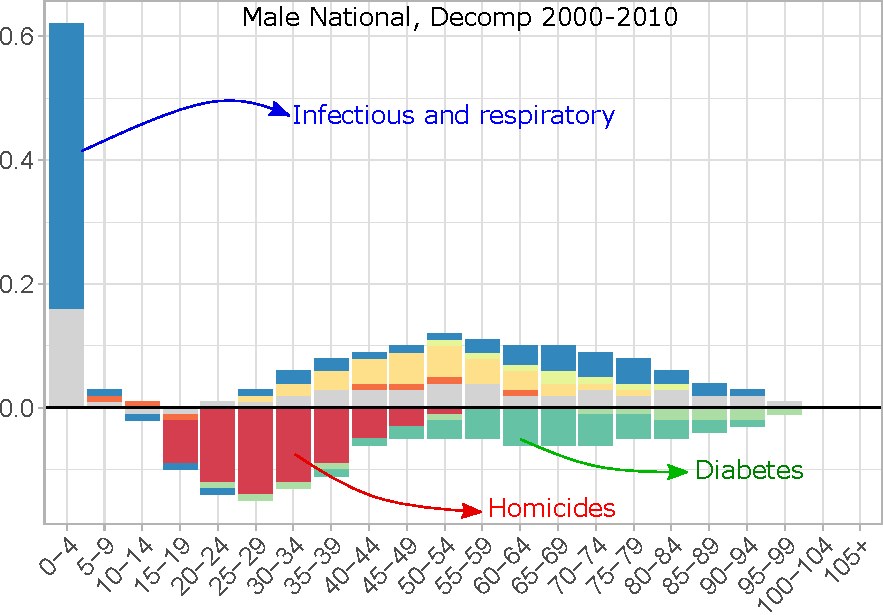
\includegraphics[scale=.55]{Figures/Fig_1}
				\end{center}
				

}
\end{frame}

\begin{frame}
\begin{center}
\Large{\textbf{10y before and after war on drugs and universal healthcare reform}}
\end{center}

\hspace*{-1cm}   
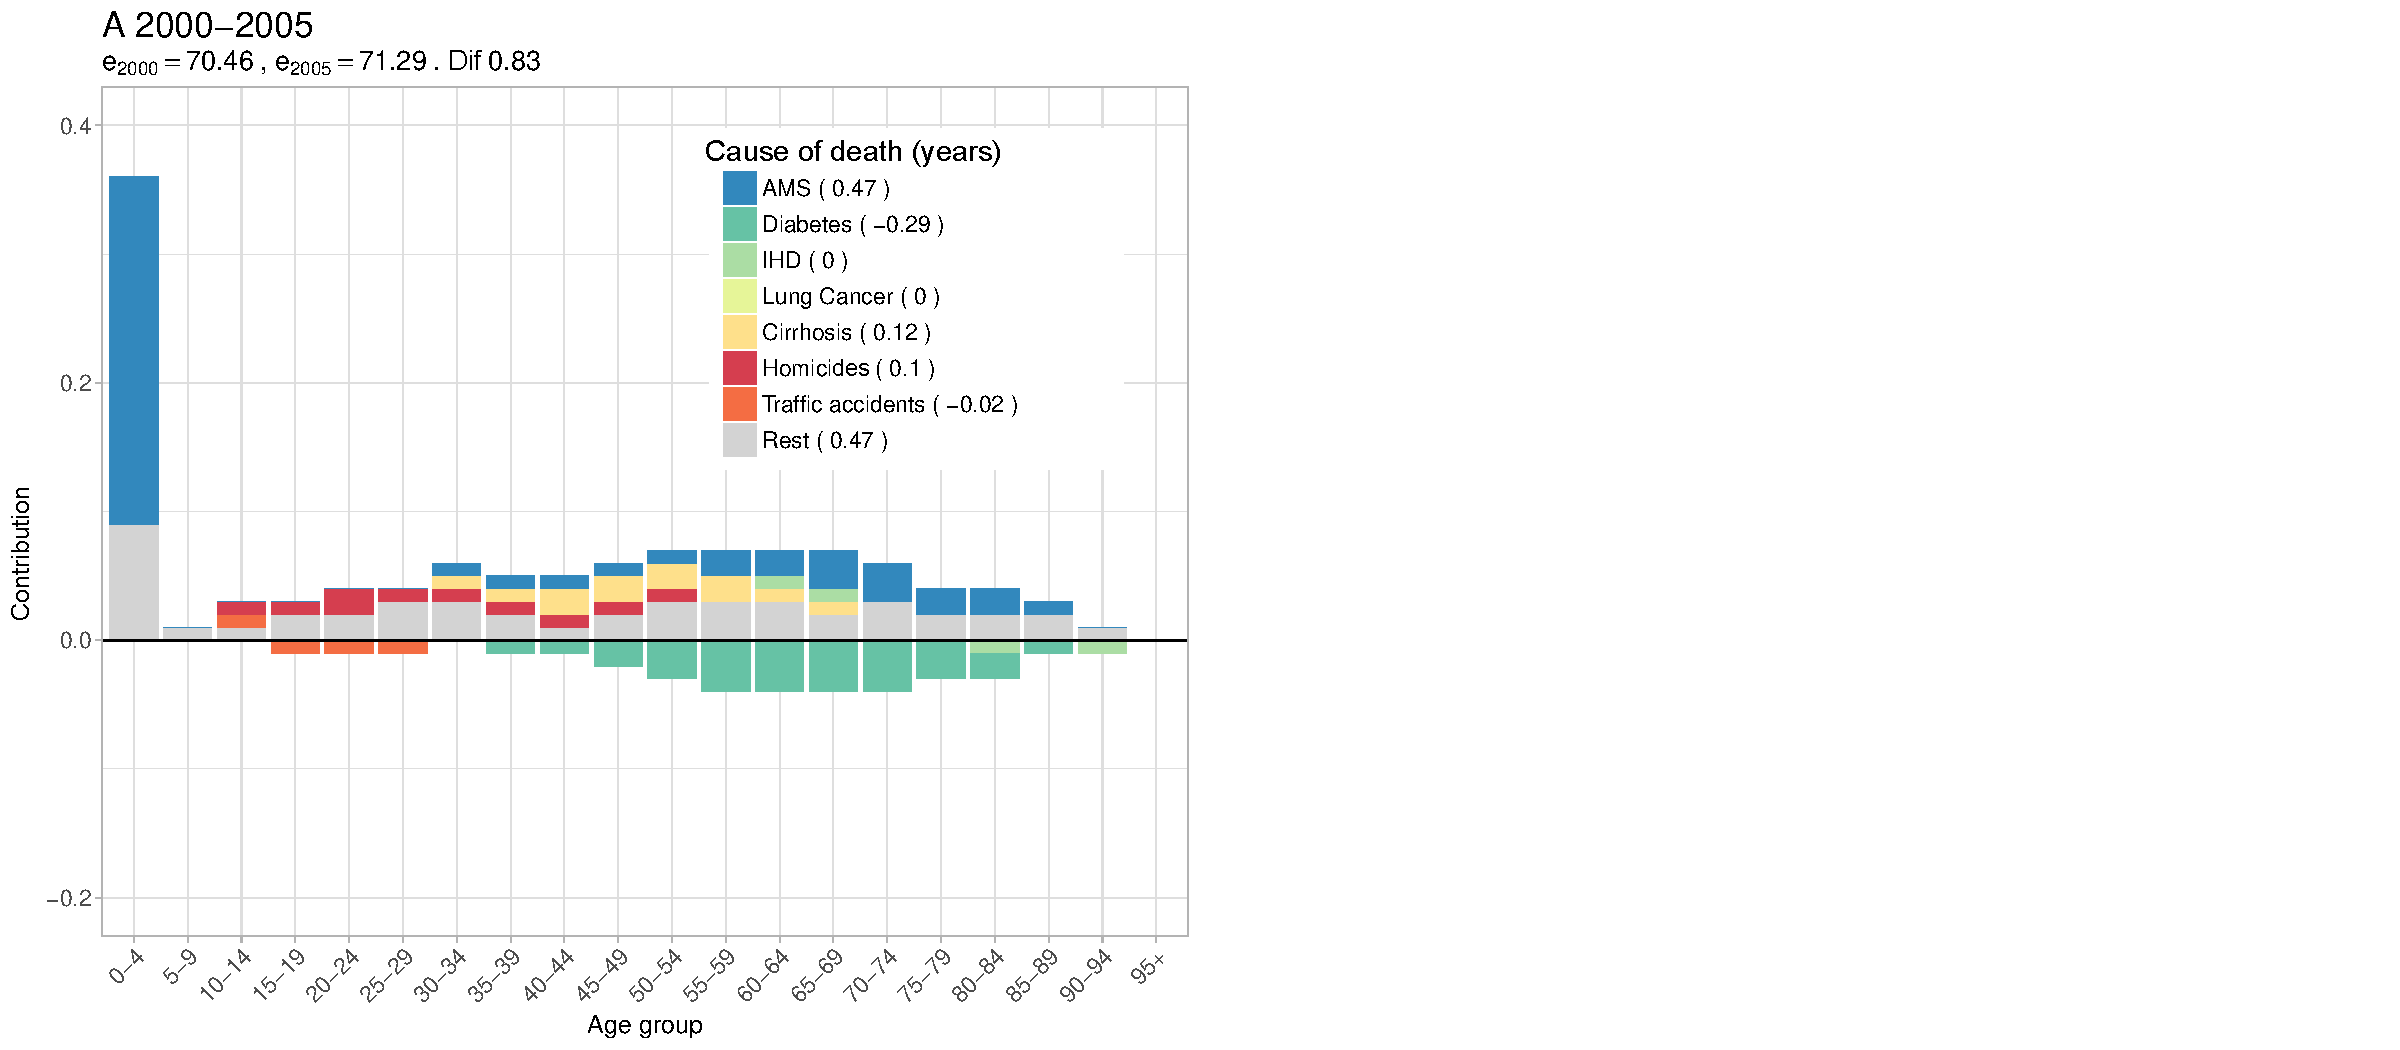
\includegraphics[scale=.31]{Figures/Fig2_1}

\end{frame}

\begin{frame}
\begin{center}
\Large{\textbf{10y before and after war on drugs and universal healthcare reform}}
\end{center}

\hspace*{-1cm}   
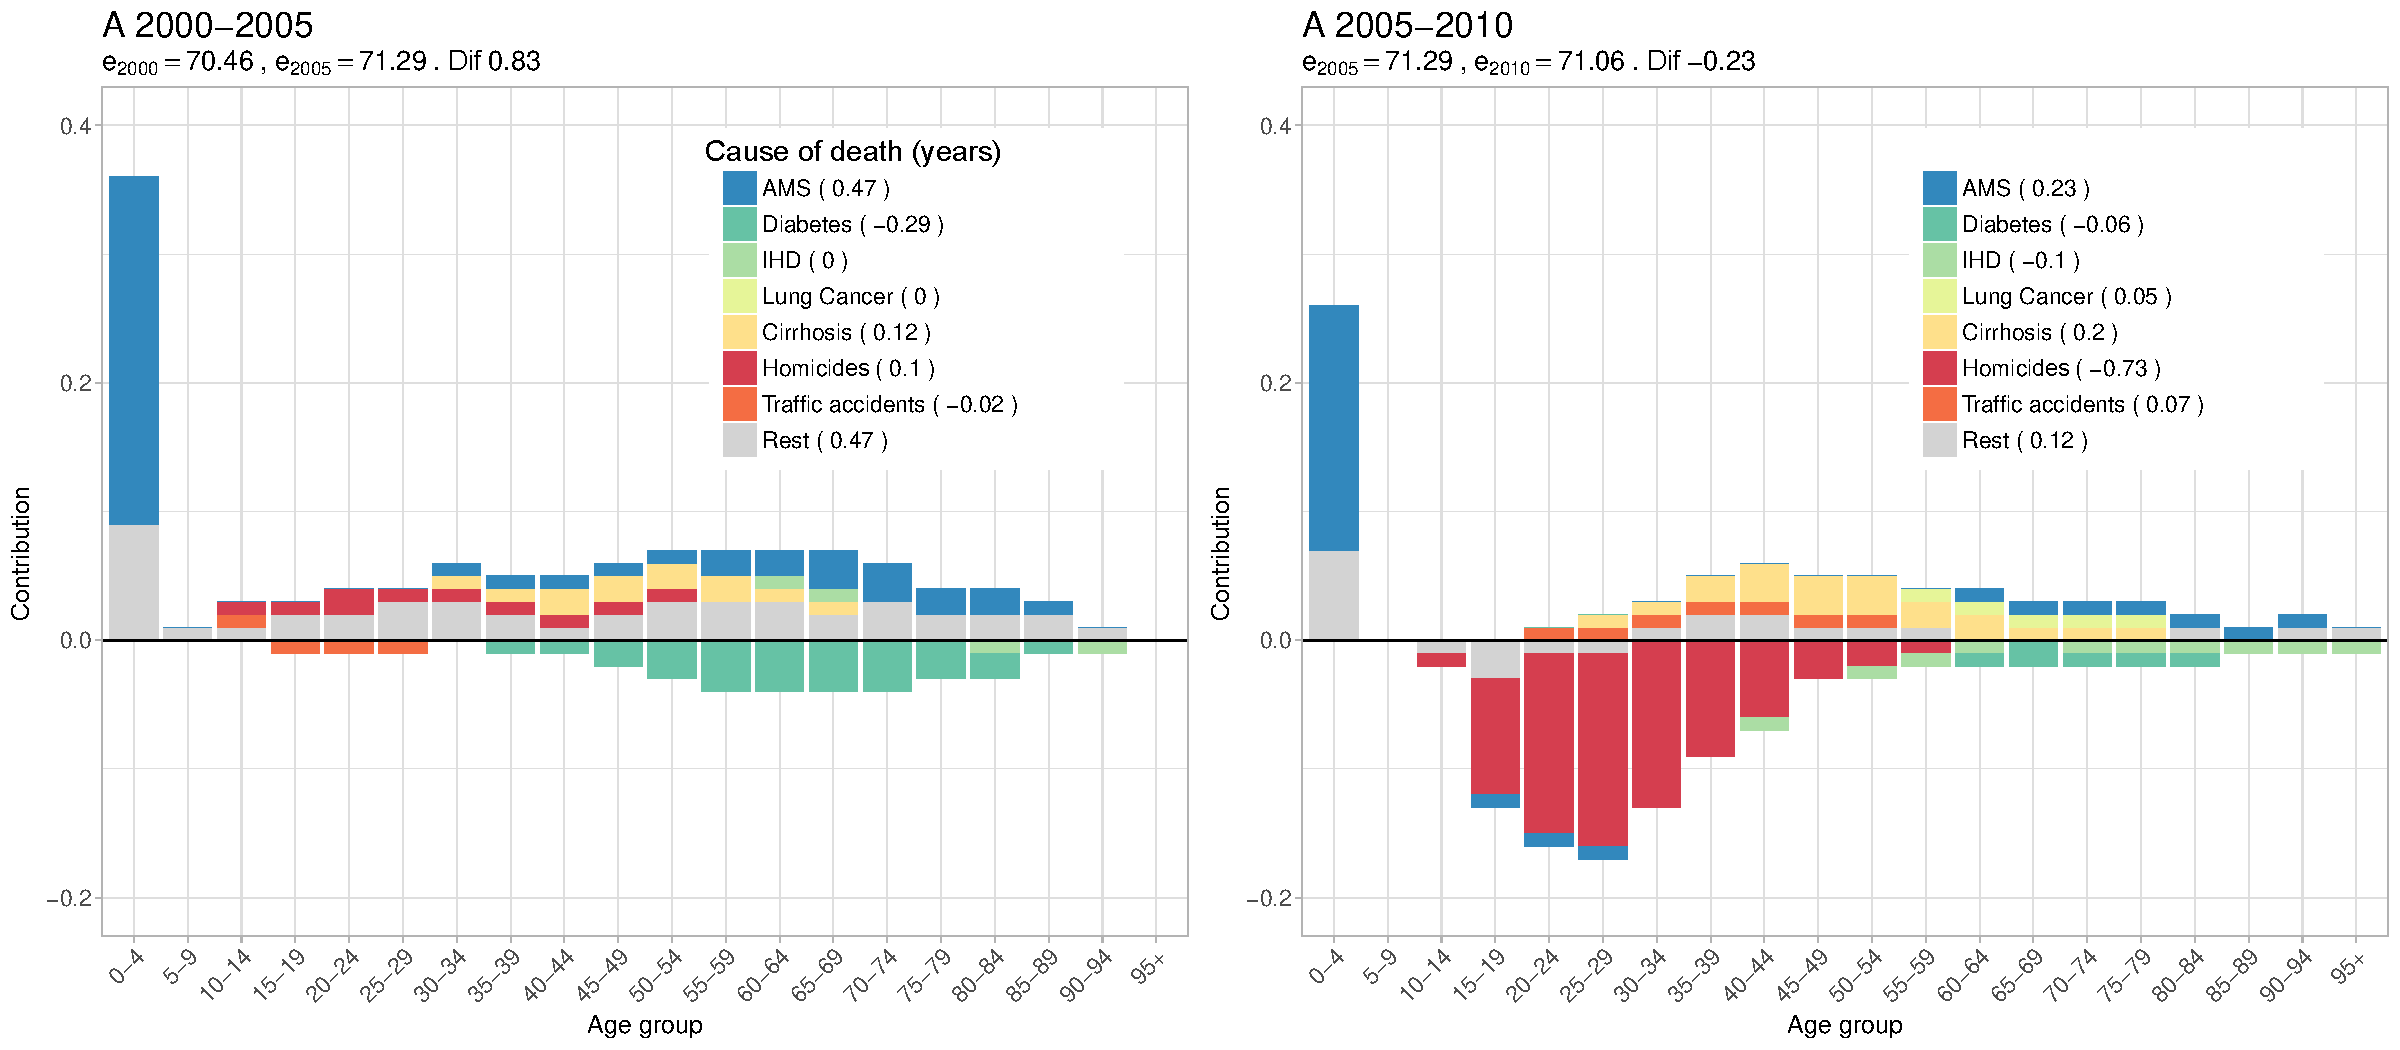
\includegraphics[scale=.31]{Figures/Fig2_2}

\end{frame}





\begin{frame}

				\begin{center}
		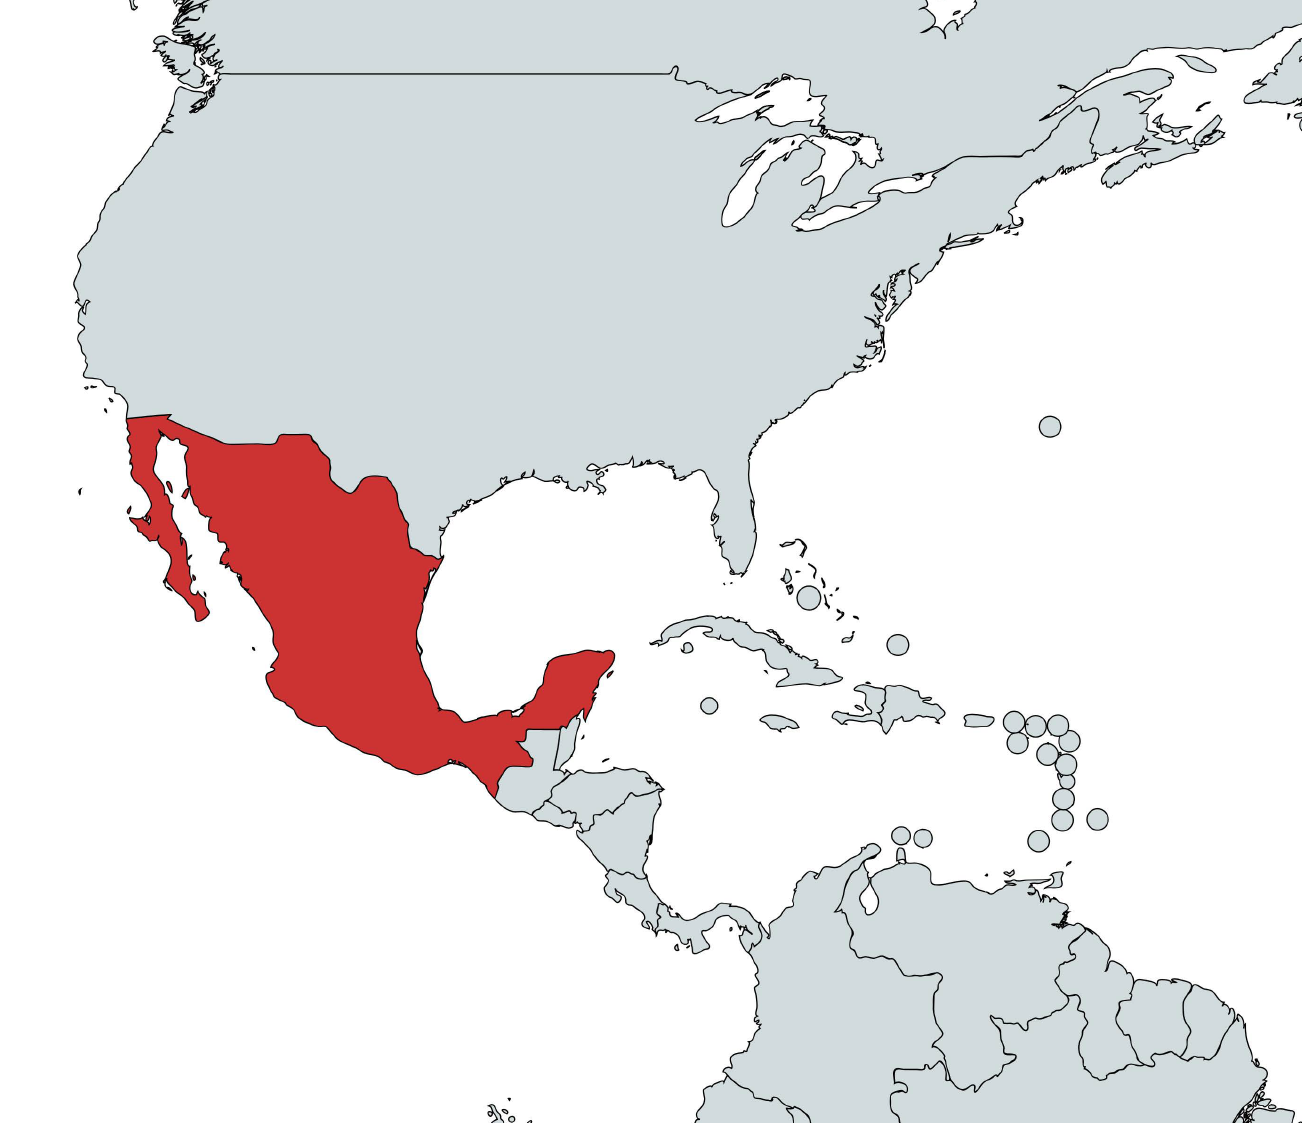
\includegraphics[scale=.3]{Figures/Mexico1}
				\end{center}
				
\end{frame}




\begin{frame}\frametitle{At the subnational level}


				\begin{center}
		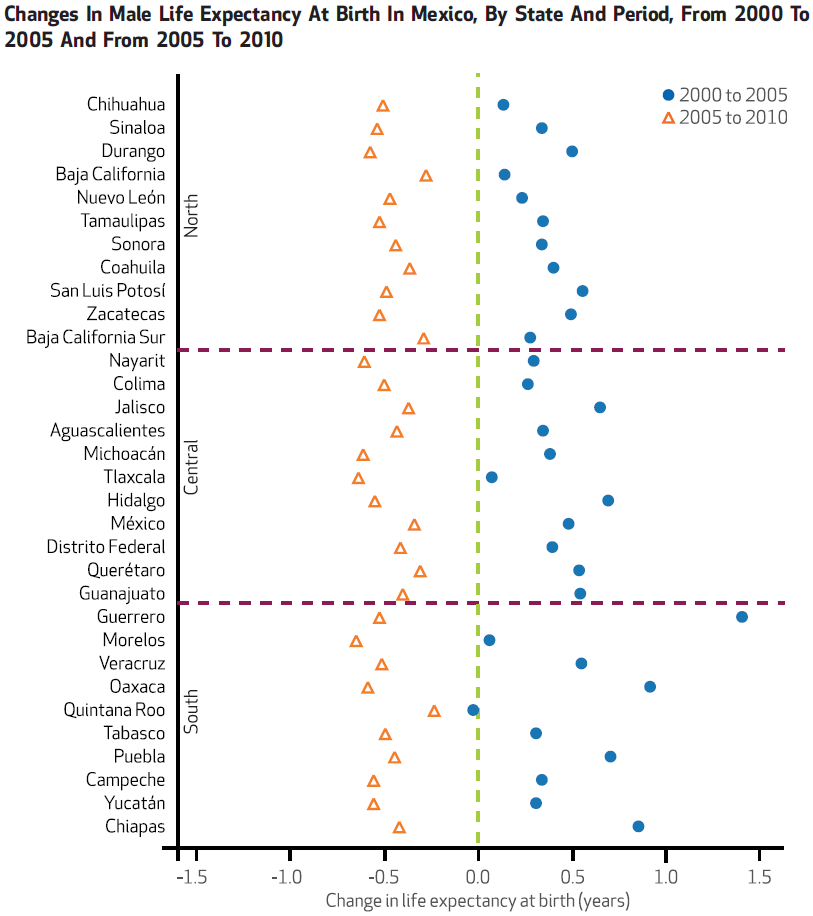
\includegraphics[scale=.37]{Figures/State_changes_e0}
				\end{center}
				
\end{frame}


\begin{frame}

\LARGE{

Gains in life expectancy due to medically amenable causes
\begin{enumerate}
\item Infectious
\item Respiratory diseases 
\item Birth conditions
\item ...
\end{enumerate}

 \pause
\begin{center}
\textbf{Wiped out by the increase of homicides after 2005 in each of the 32 states in Mexico}
\end{center}				

}
\end{frame}


\begin{frame}
\LARGE{
Why lifespan variation \pause in the context of rising violence?
\pause
		\begin{itemize}
		
		\item Links to individuals' \textbf{decisions} (expected lifetime and uncertainty). \pause

		\item \textbf{Uncertain times} lead to change in behavior. \pause
		
		\item Homicides affect mainly \textbf{young men}. \pause
		
		\item State of \textbf{vulnerability}
						
		\end{itemize}

}
\end{frame}



\begin{frame}
\Large{
We use the concept of \textbf{``Avoidable/Amenable"} mortality:
%An approach to approximate the impact of healthcare and other interventions, and to reveal potential areas of improvement. Based on causes that should not occur in the presence of effective and timely healthcare.
		\begin{enumerate}
		
		
\color{blue} 		\item Amenable to medical intervention \begin{tiny}Infectious \& respiratory \end{tiny}

\pause

\color{ForestGreen}		\item Diabetes
		
		\item Ischemic heart diseases (IHD)
		
		\item Lung cancer.
		 
		\item Cirrhosis.
		
\pause
		
\color{red}		\item \textbf{Homicide}
		
\color{yellow}		\item Road traffic accidents
		
		\pause
		
\color{gray}				\item Rest.

		
		\end{enumerate}			

}
\end{frame}


\begin{frame}

\Large{
\textbf{$e^{\dagger}_{15}\longrightarrow  $ }average remaining life expectancy when death occurs.

\begin{itemize}
\item Easy \textbf{public health interpretation}.
\pause
\item \textbf{Quantify} age and cause specific effects.
\pause
\item Separate ages that \textbf{decrease} from those that \textbf{increase}.
\pause
\item Conditioned to age 15 to capture the \textbf{onset of violence}.
\end{itemize}

}
\end{frame}




\begin{frame}
\begin{center}
\Large{\textbf{National life expectancy}}
\end{center}

\hspace*{-1cm}   
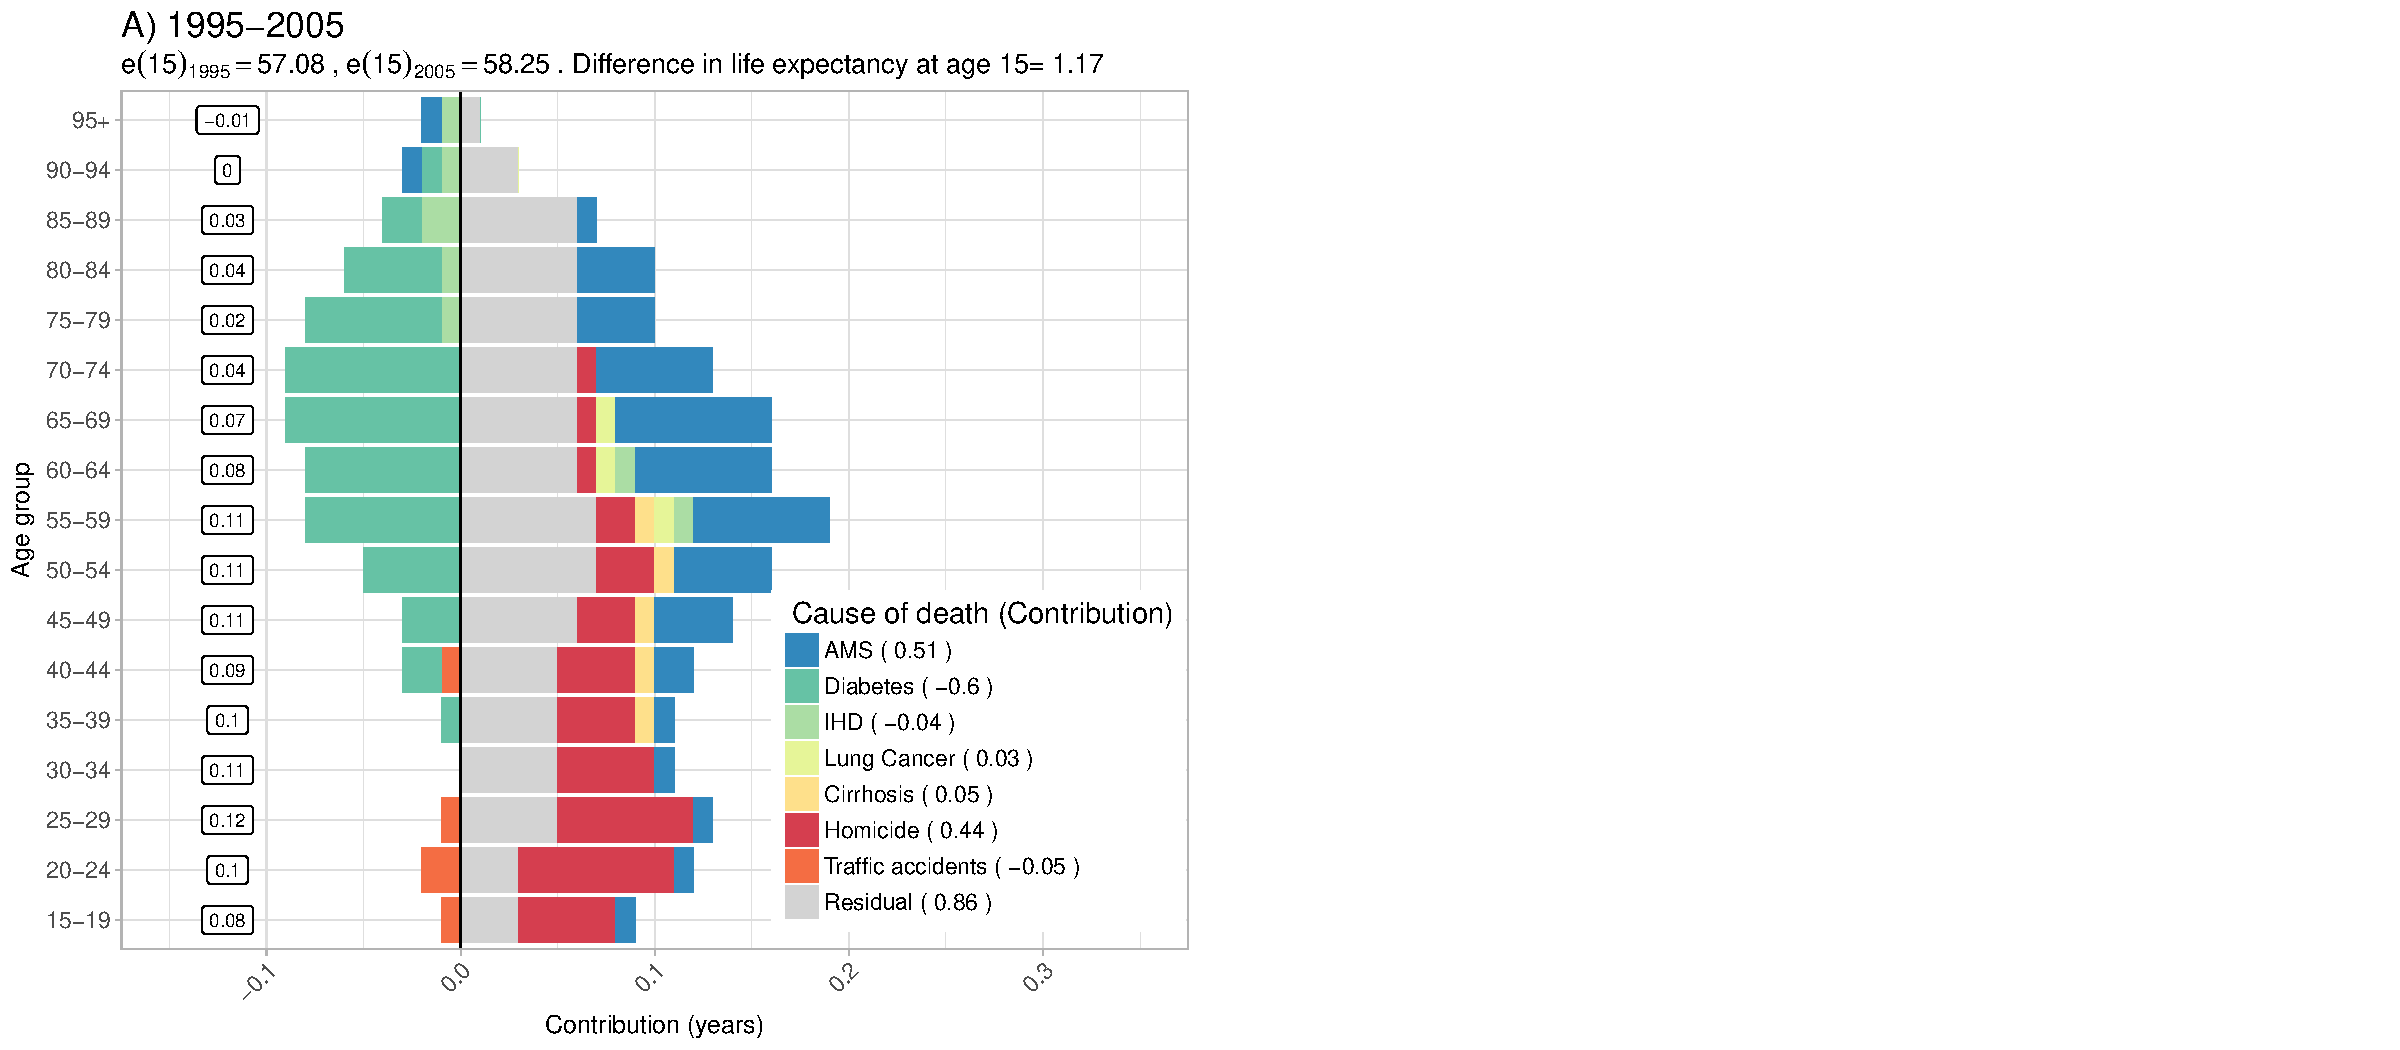
\includegraphics[scale=.31]{Figures/Figure_1_2}

\end{frame}


\begin{frame}
\begin{center}
\Large{\textbf{National life expectancy}}
\end{center}

\hspace*{-1cm}   
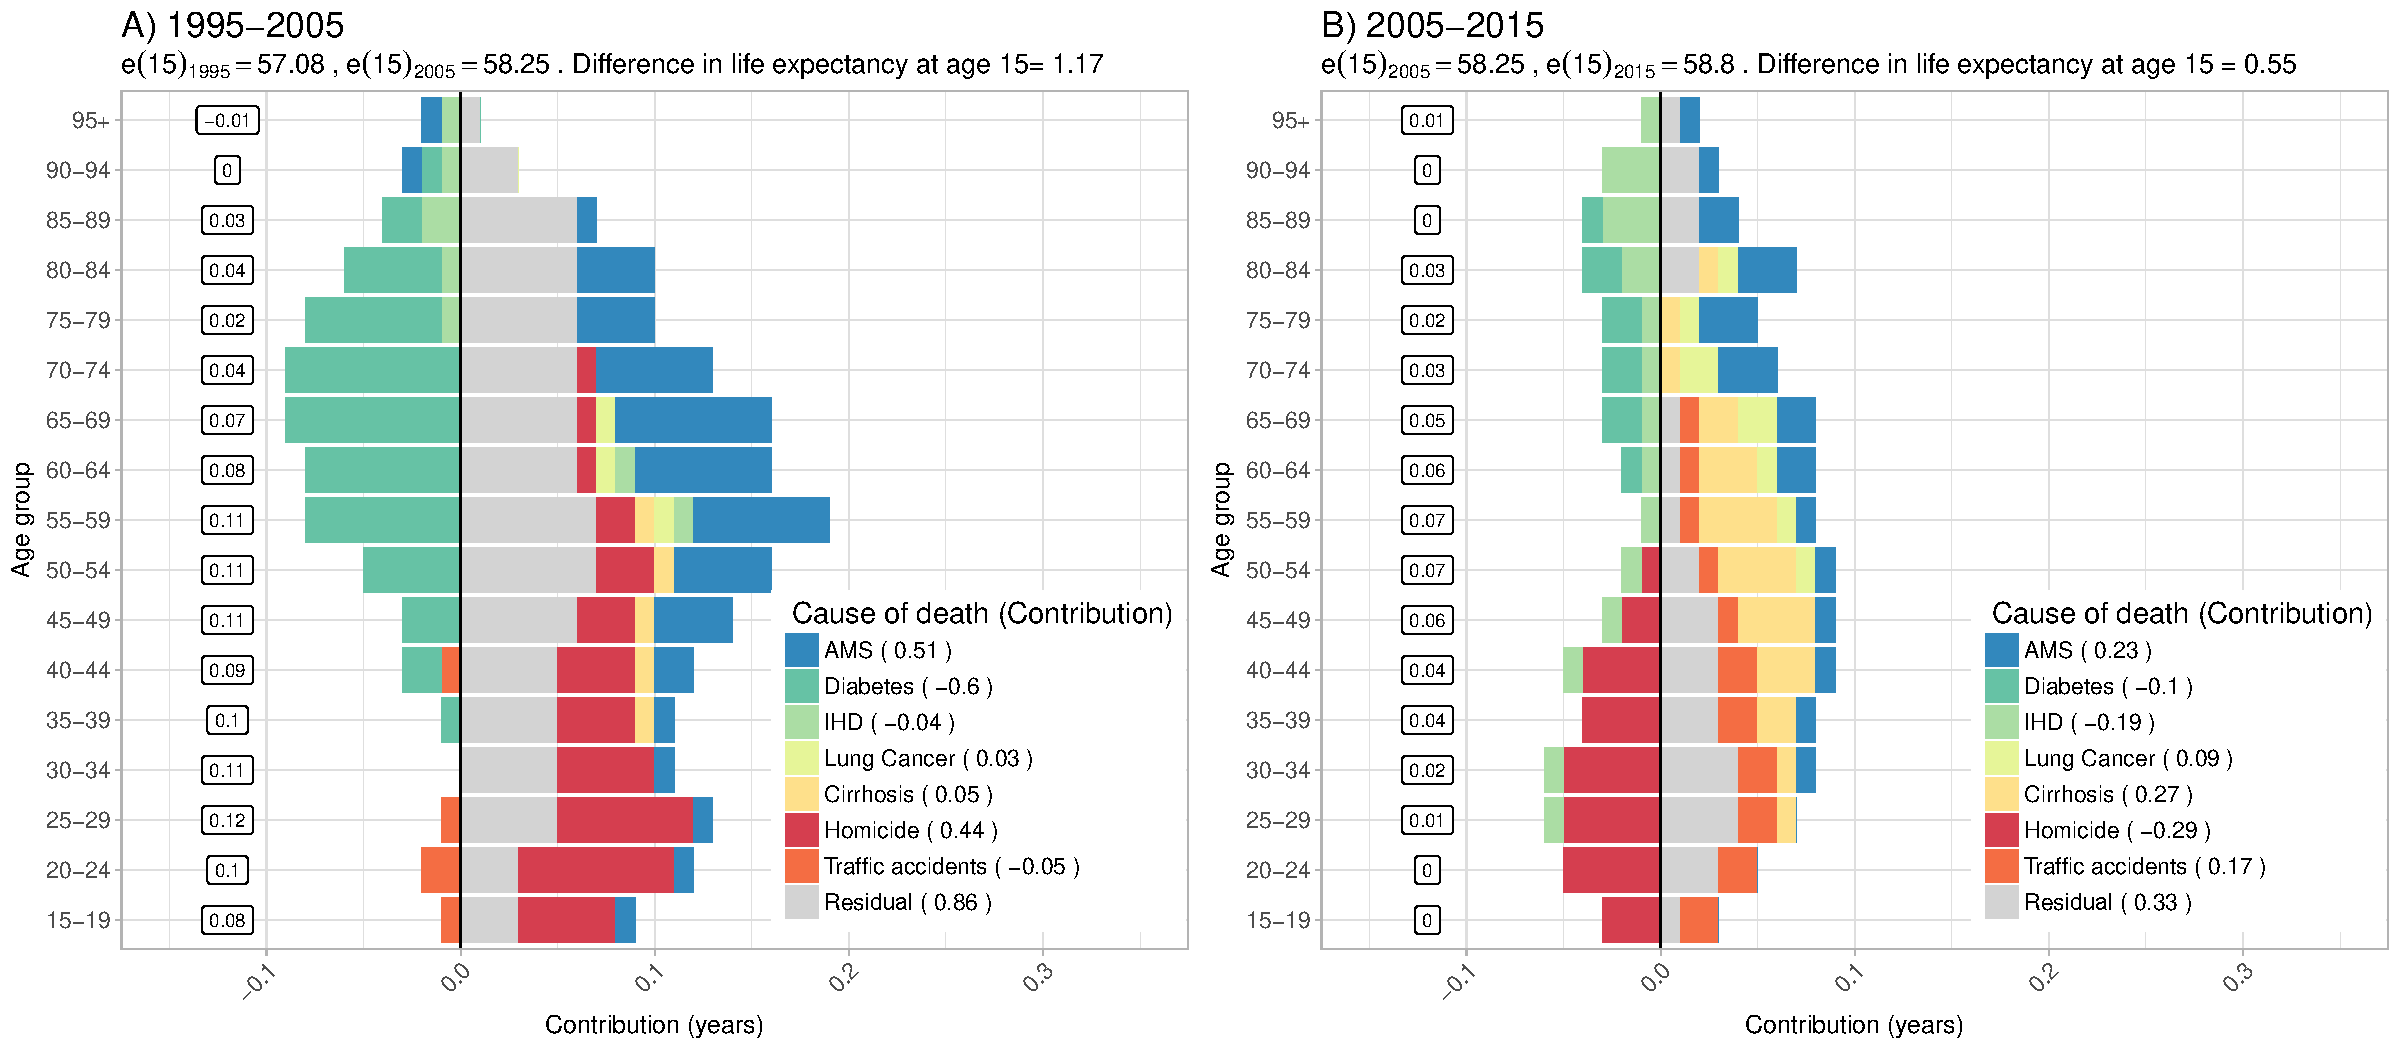
\includegraphics[scale=.31]{Figures/Figure_1}

\end{frame}


\begin{frame}
\begin{center}
\Large{\textbf{National lifespan inequality}}
\end{center}

\hspace*{-1cm}   
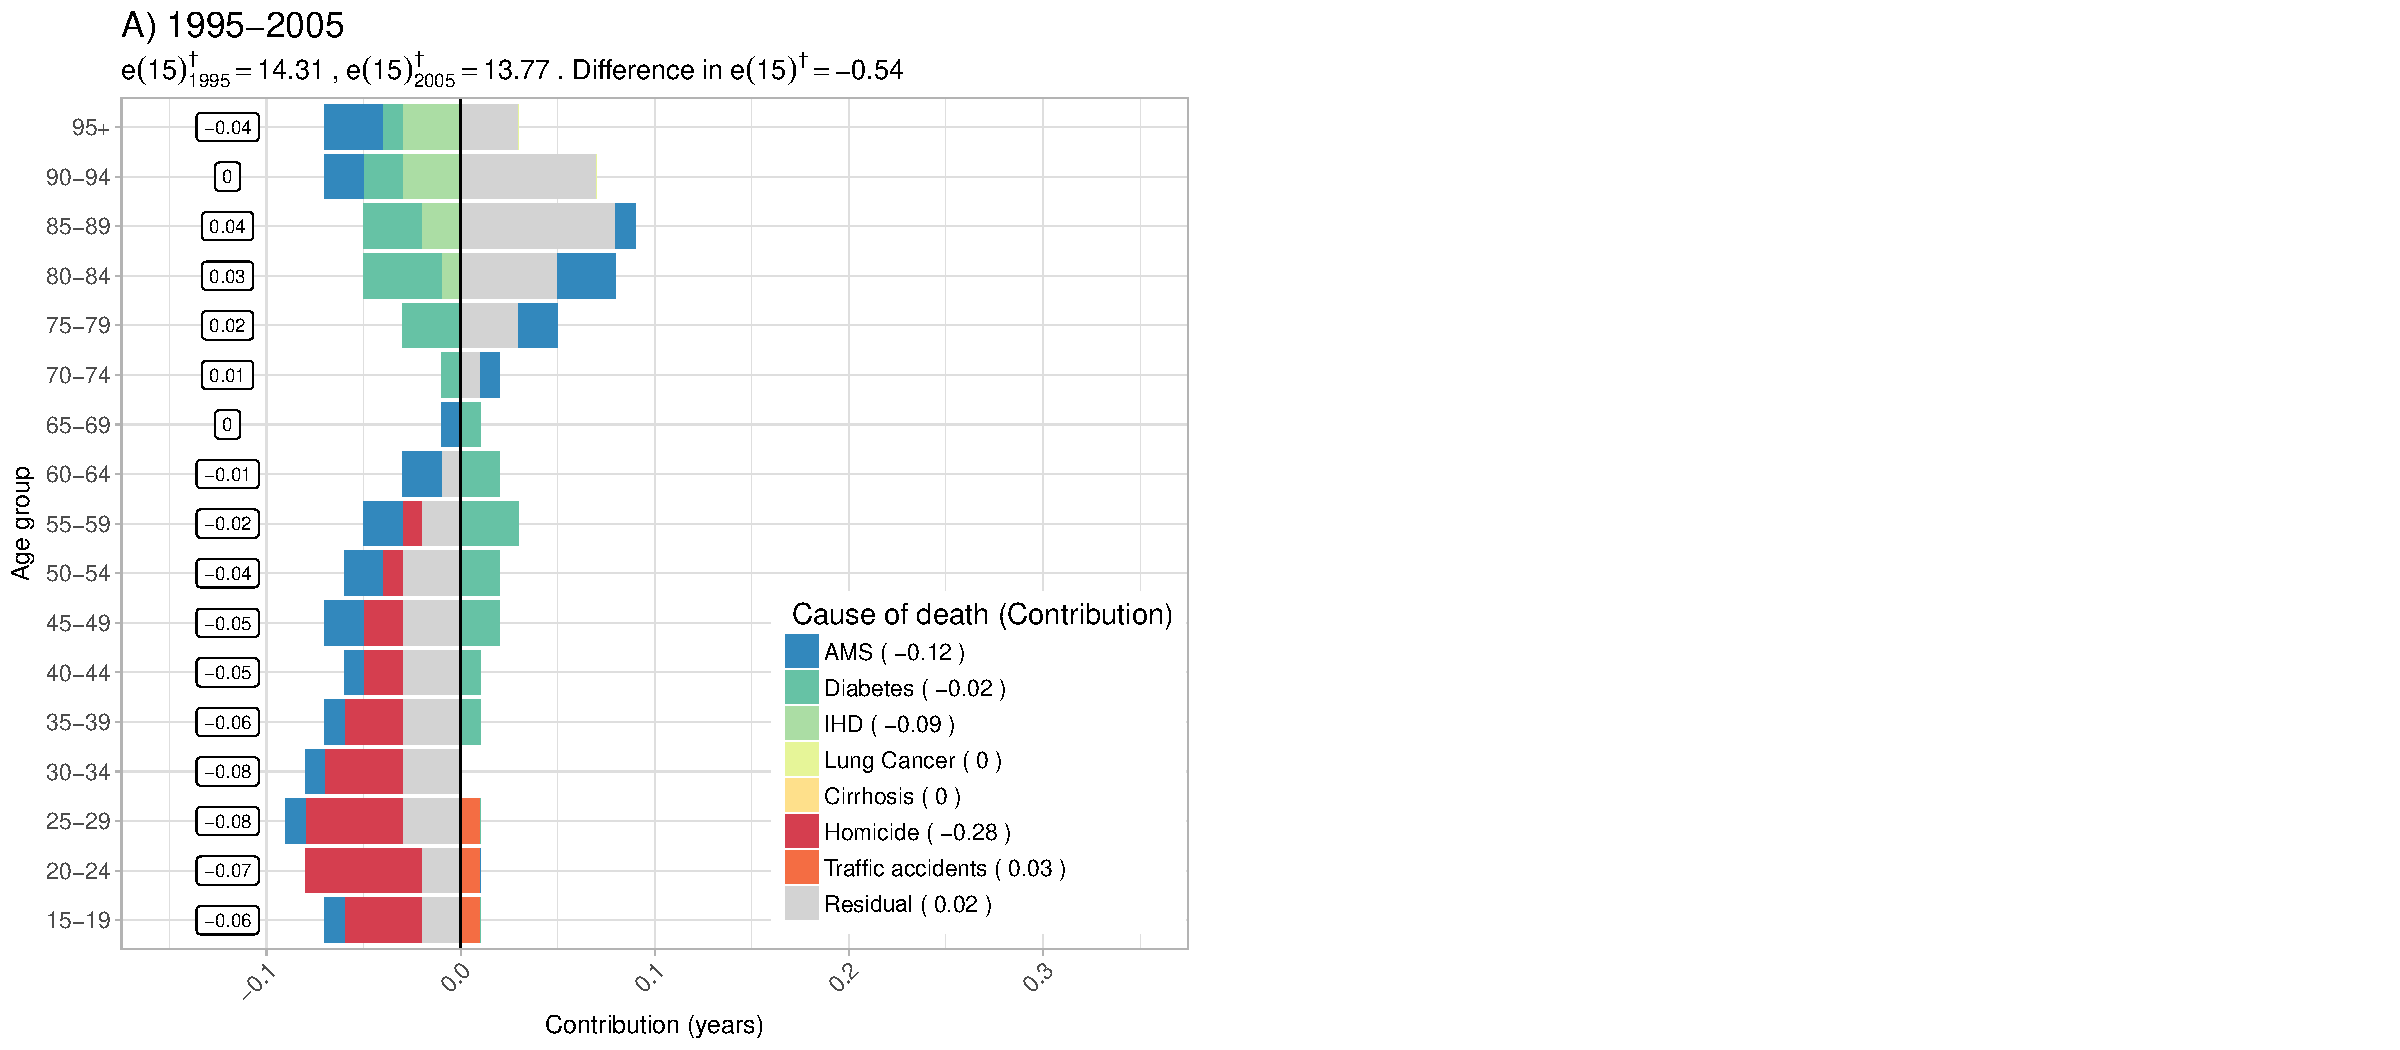
\includegraphics[scale=.31]{Figures/Figure_2_2}

\end{frame}


\begin{frame}
\begin{center}
\Large{\textbf{National lifespan inequality}}
\end{center}

\hspace*{-1cm}   
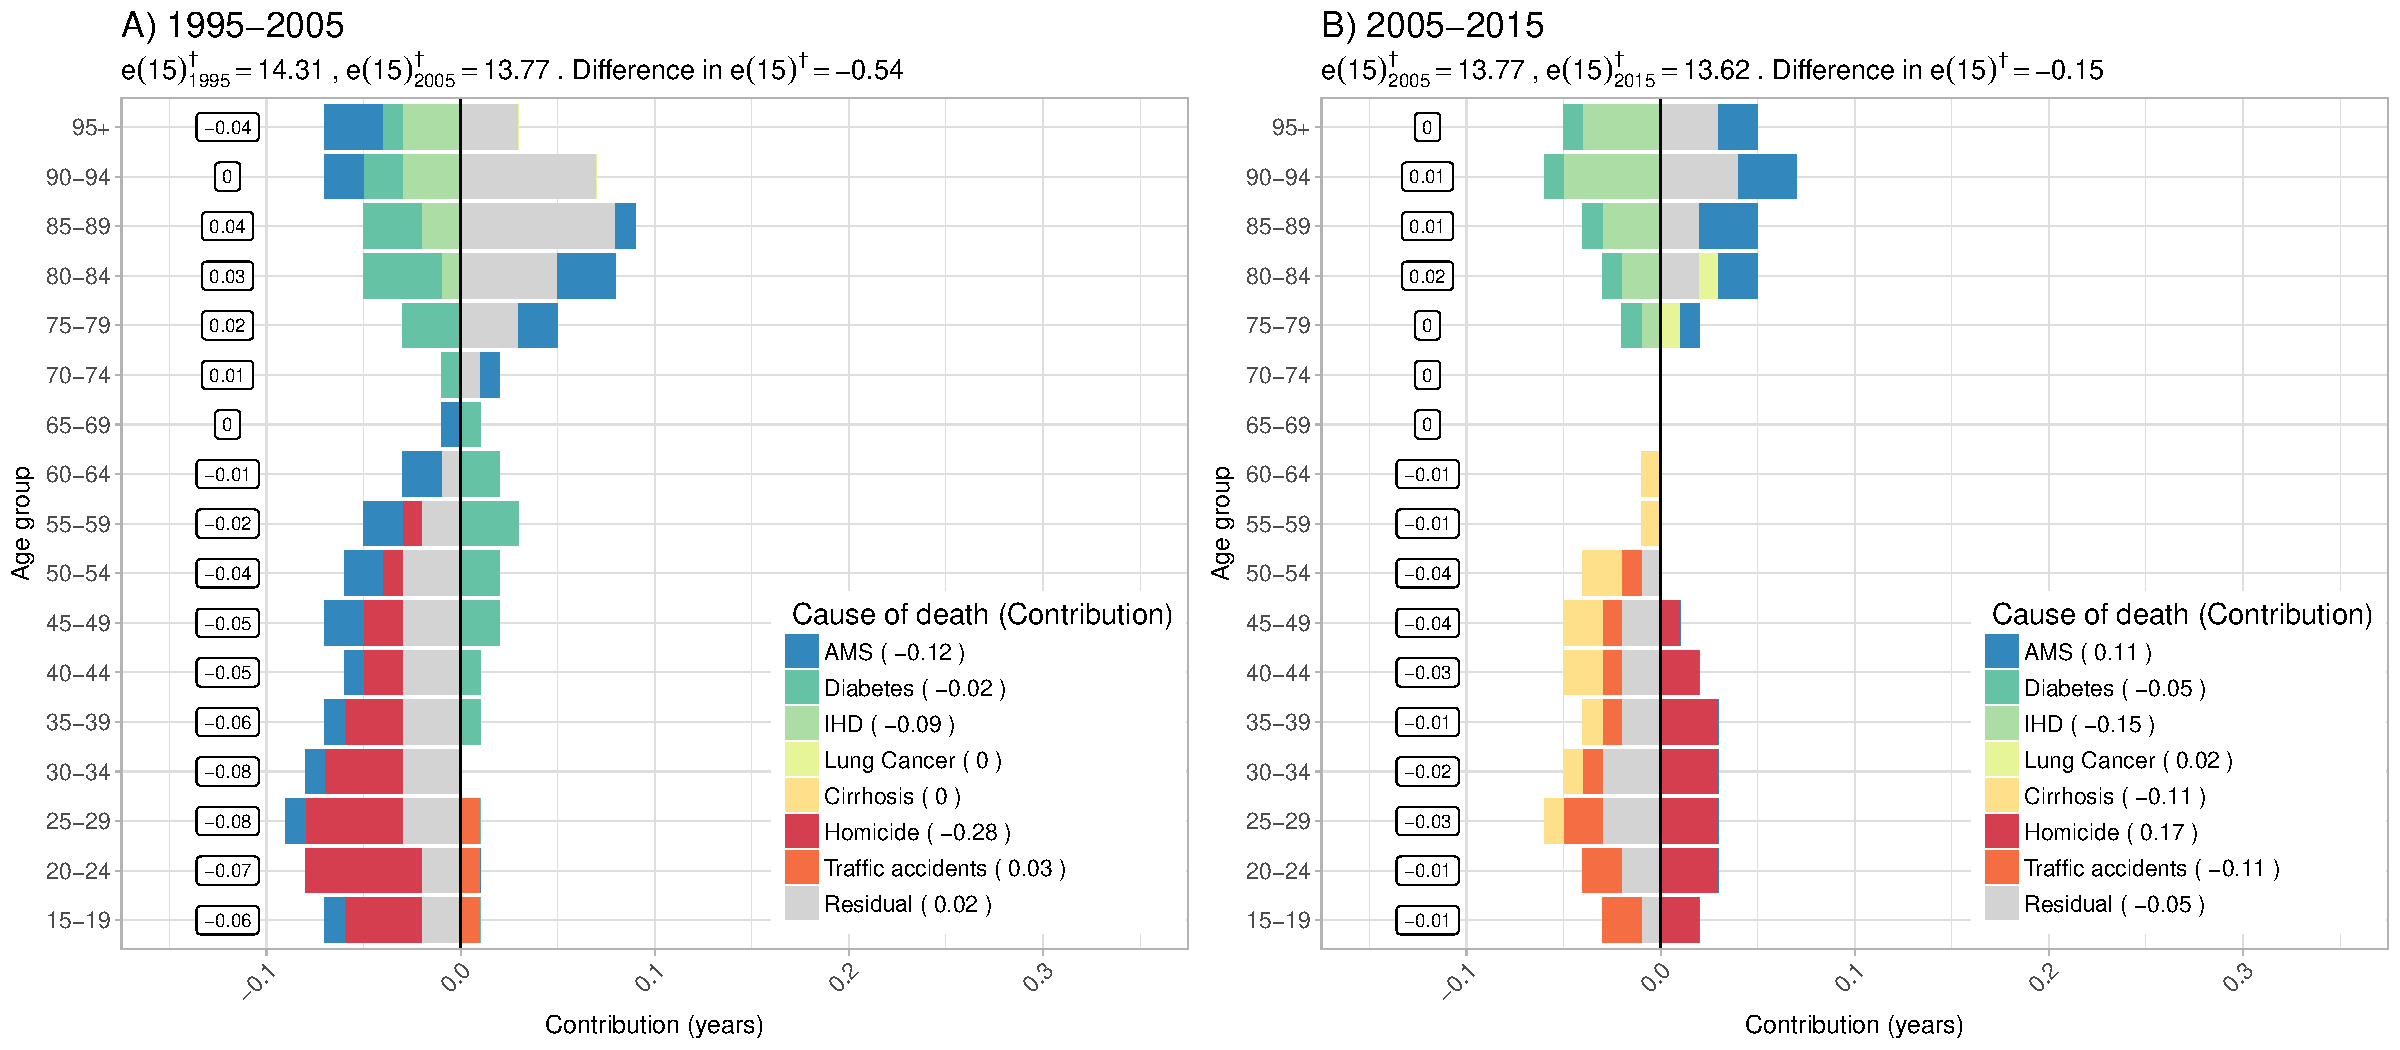
\includegraphics[scale=.31]{Figures/Figure_2}

\end{frame}

\begin{frame}
\begin{center}
\Large{\textbf{Homicides not evenly shared across Mexico}}
\end{center}

\hspace*{-1cm}   
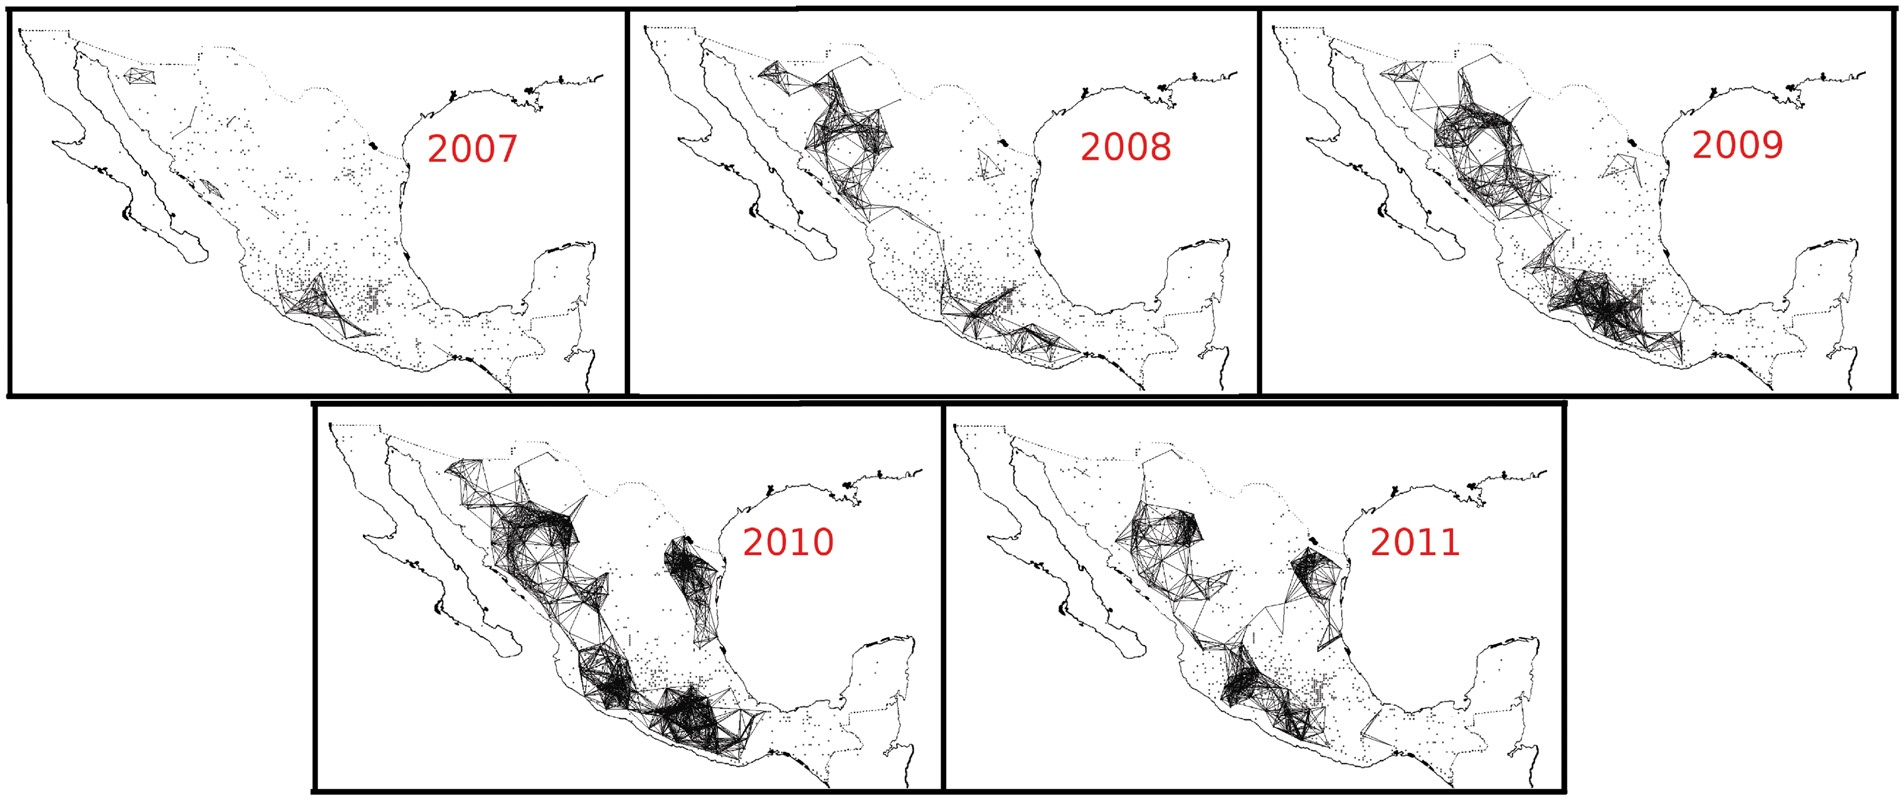
\includegraphics[scale=.78]{Figures/map1}

\end{frame}

\begin{frame}
\begin{center}
\Large{\textbf{Subnational level}}
\end{center}

\hspace*{-1cm}   
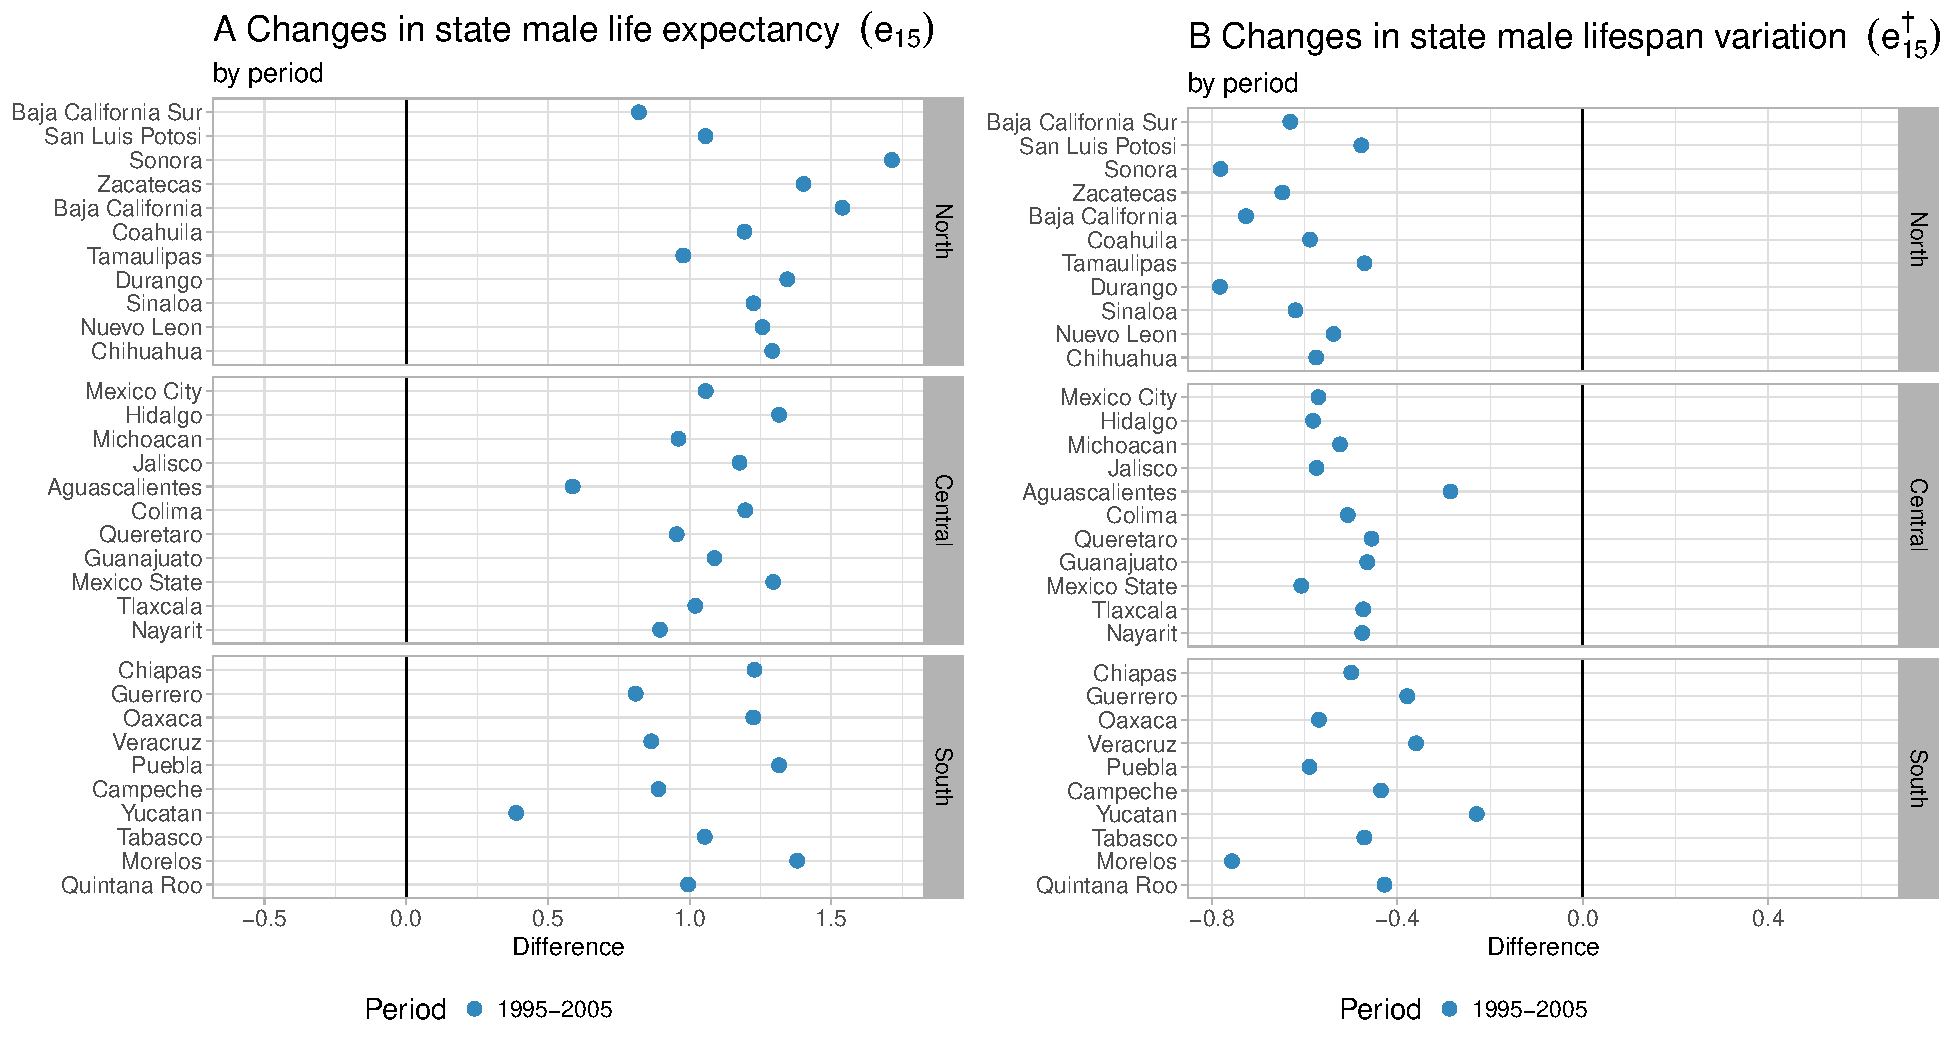
\includegraphics[scale=.38]{Figures/Figure_3_1}

\end{frame}


\begin{frame}
\begin{center}
\Large{\textbf{Subnational level}}
\end{center}

\hspace*{-1cm}   
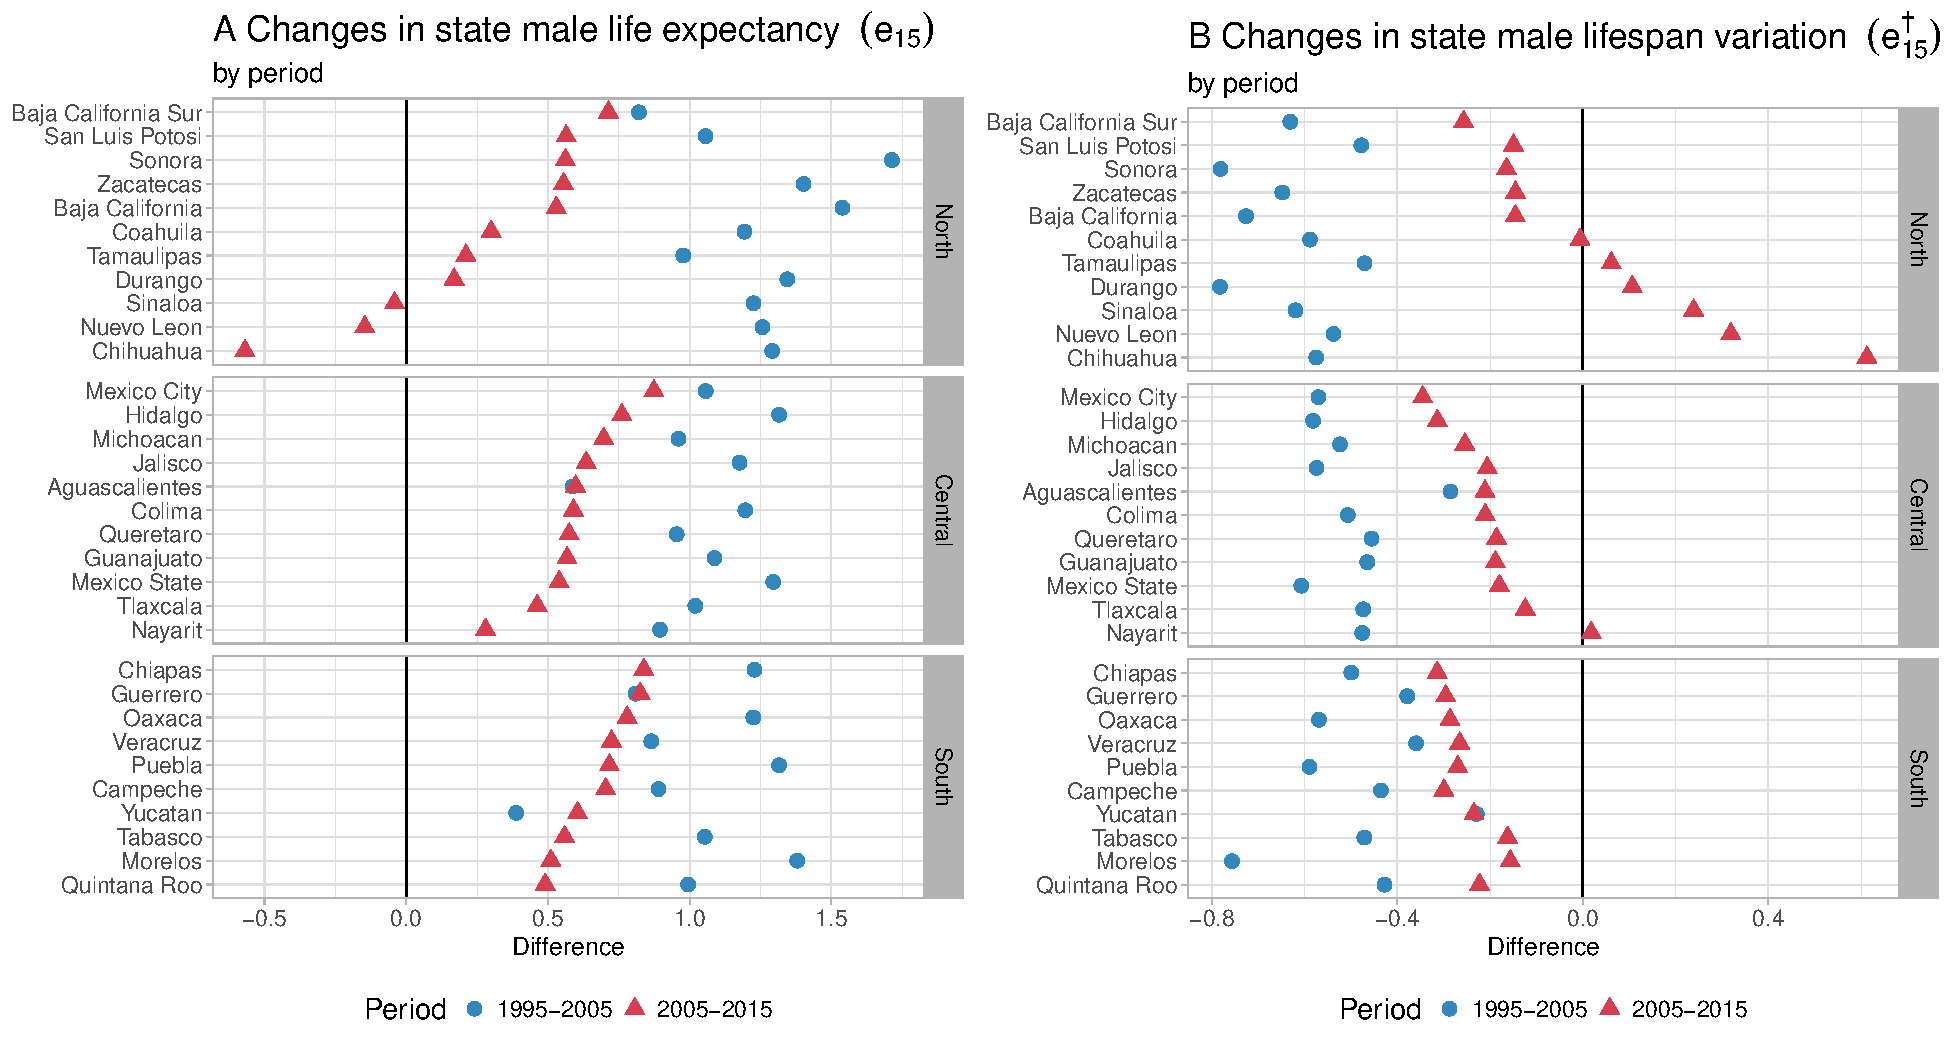
\includegraphics[scale=.38]{Figures/Figure_3}

\end{frame}



\begin{frame}

\Large{
Chihuahua (Bordering with Texas): Rates 3 times those of US troops in Iraq between 2003 and 2006!
				\begin{center}
		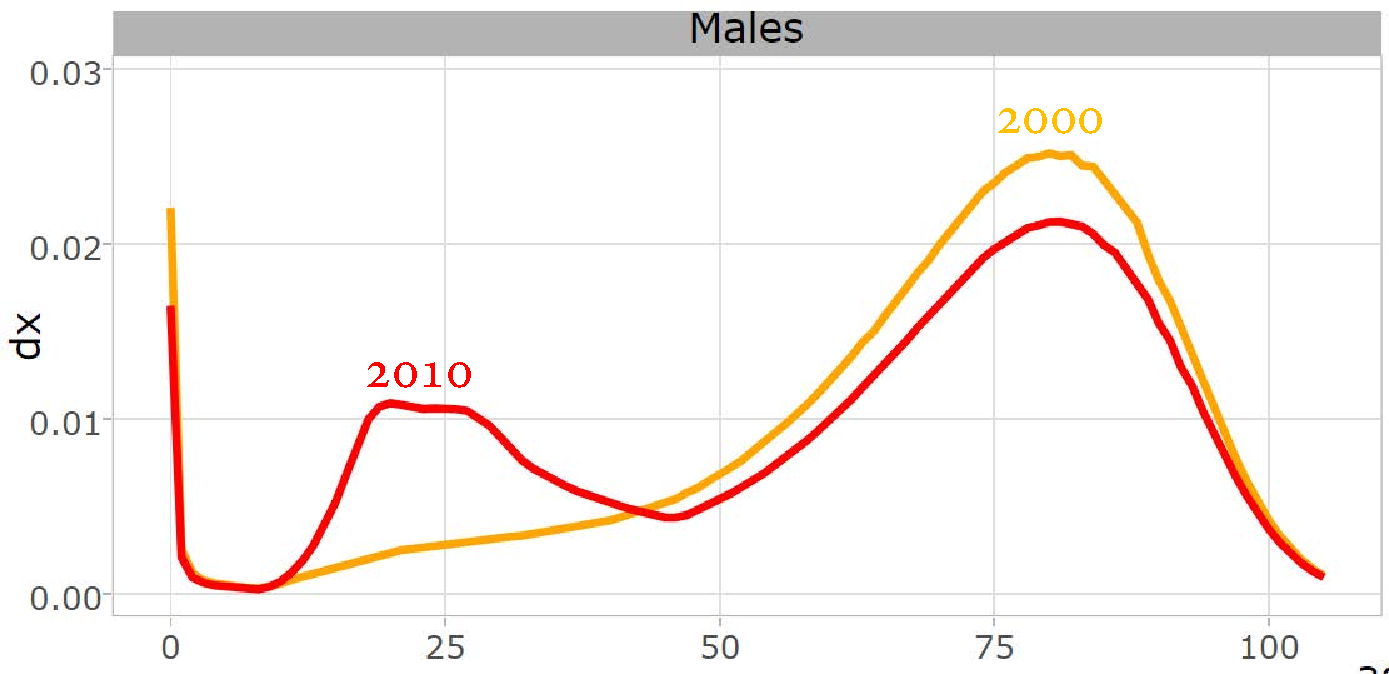
\includegraphics[scale=.45]{Figures/Distr_chihuahua}
				\end{center}				

}
\end{frame}



\begin{frame}
\begin{center}
\Large{\textbf{Cause-specific results}}
\end{center}

\hspace*{-1cm}   
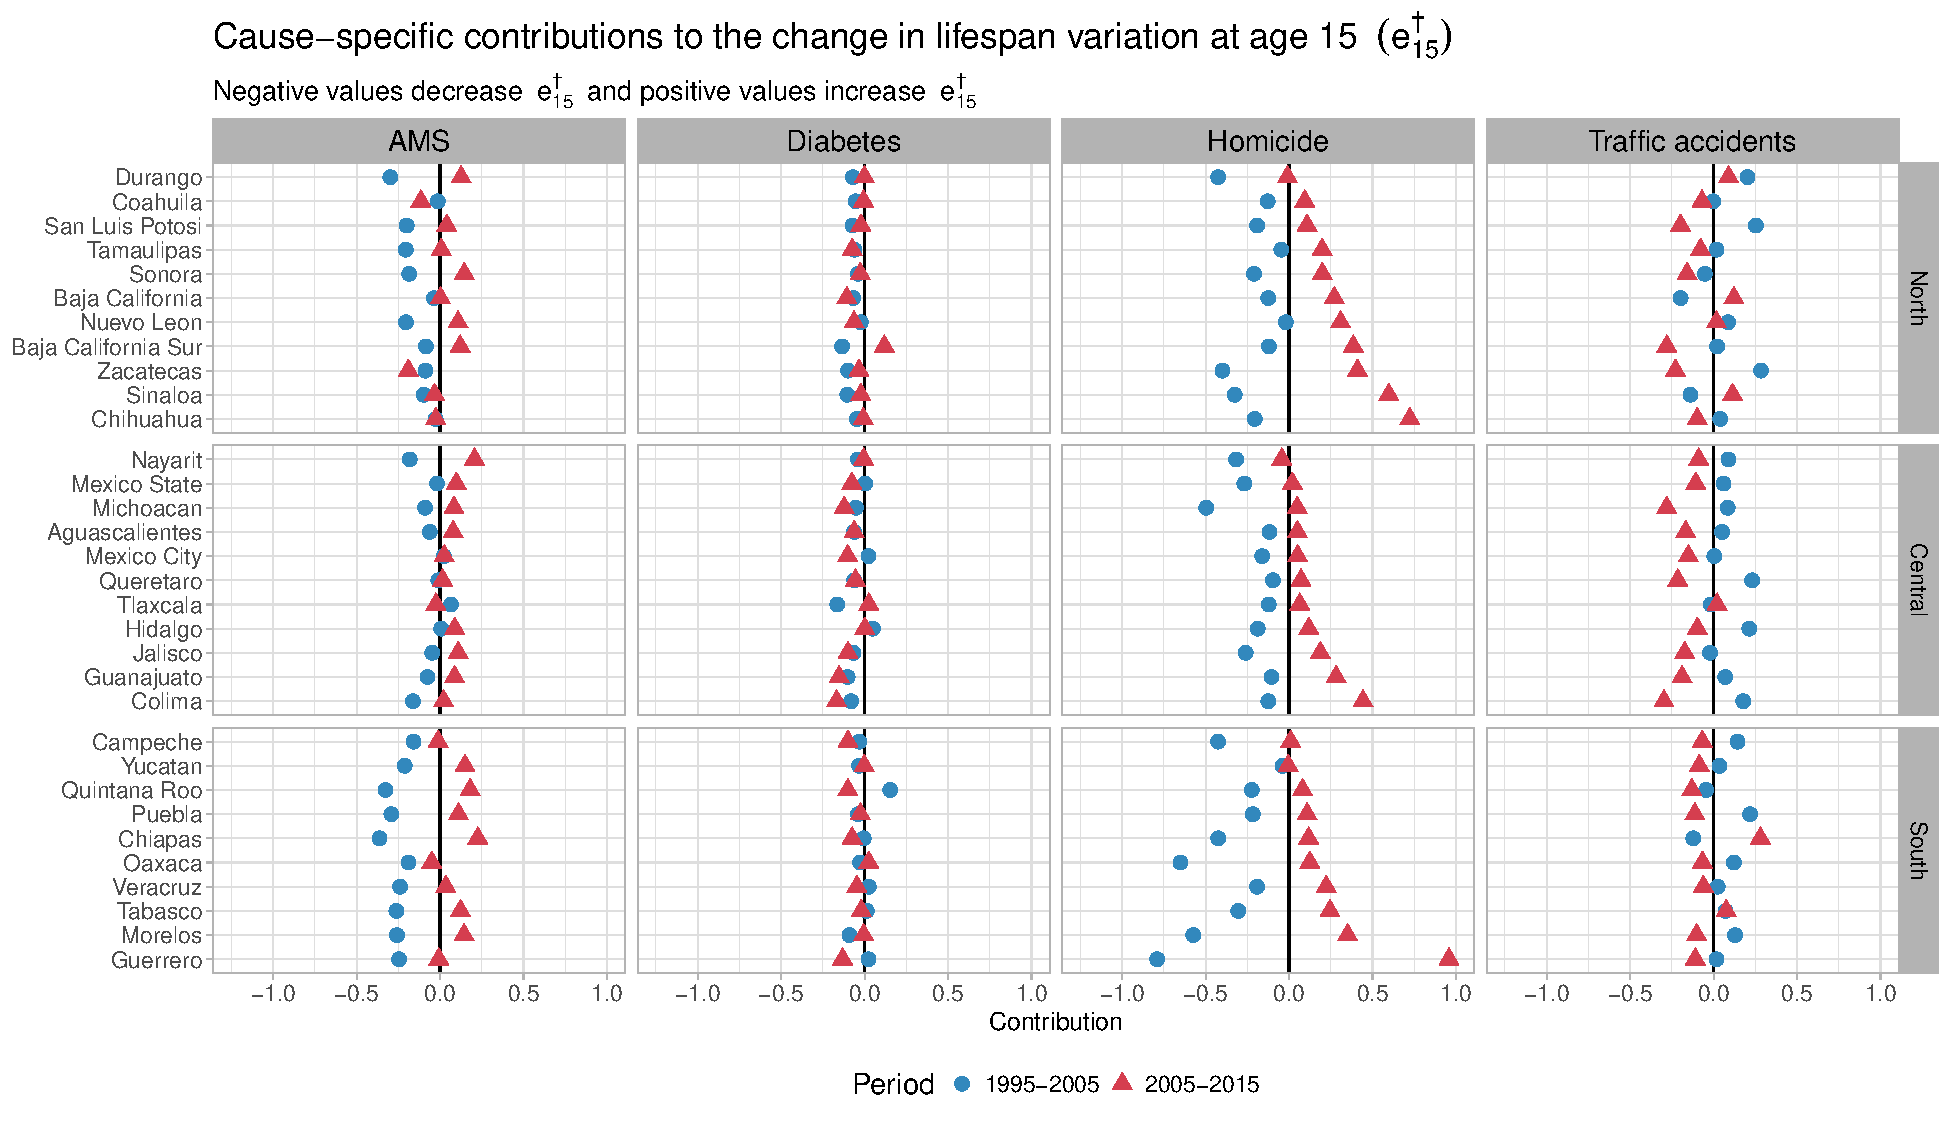
\includegraphics[scale=.38]{Figures/Figure_4}

\end{frame}


\begin{frame}

\Large{
2 of most dangerous cities in the world in 2016 in this state (The Economist)!

				\begin{center}
		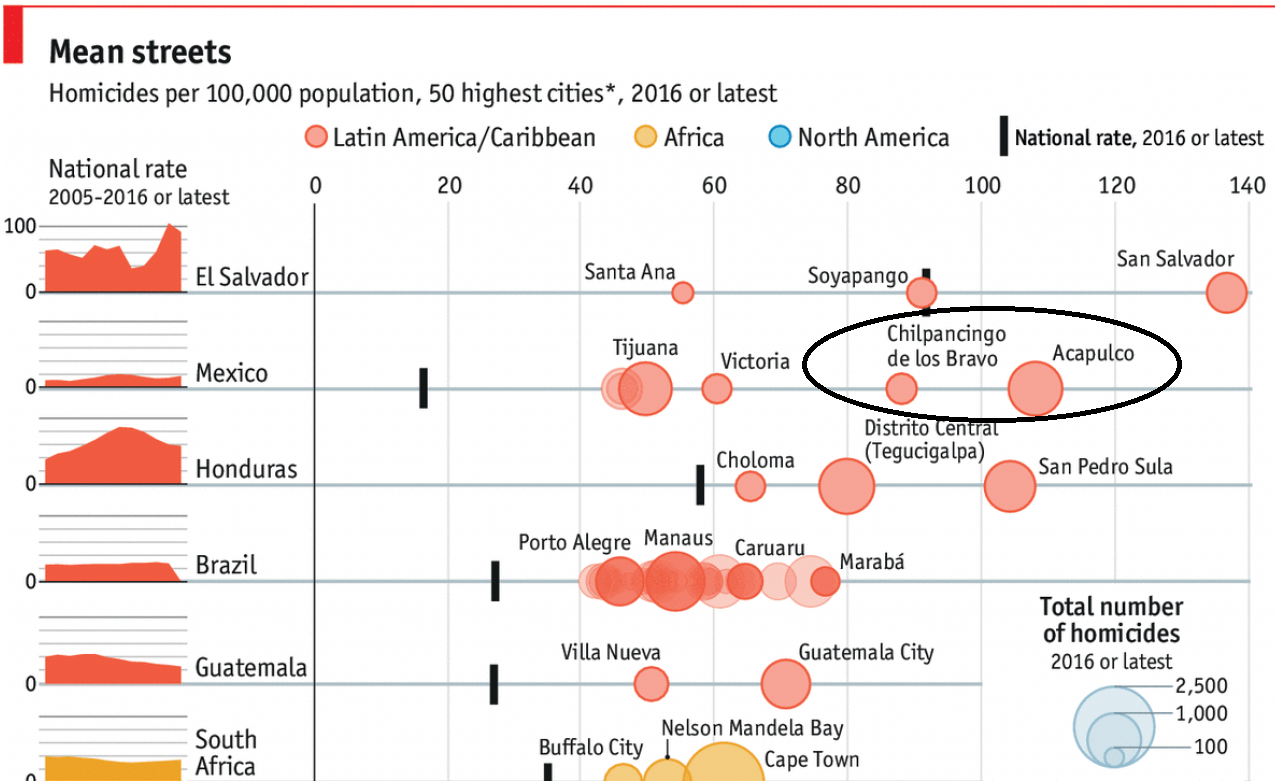
\includegraphics[scale=.38]{Figures/Capture}
				\end{center}				

}
\end{frame}


\begin{frame}
\Huge{
\begin{center}
International Perspective \linebreak \\

{\fontsize{70}{80}\selectfont 

 $\backsim$ 2,000,000}\\
15-30

\end{center}
}
\end{frame}

\begin{frame}
\Huge{
\begin{center}
{\fontsize{70}{80}\selectfont 77\%}\\
Men

\end{center}
}
\end{frame}


\begin{frame}
\Huge{
\begin{center}
{\fontsize{70}{80}\selectfont 35\% Homicides}\\
(+ 1/2 million)

\end{center}
}
\end{frame}


\begin{frame}
\Large{
Key messages \pause

		\begin{itemize}
		
		\item Homicides \textbf{reversed} life expectancy gains and increased inequality of lifespans. \pause

		\item \textbf{After 10y} of the war on drugs Mexico has not been able to go back to \textbf{2005 levels}. \pause
		
		\item Young males in Mexico \textbf{live less}, on average, and \textbf{face more uncertainty}.\pause
		
		\item \textbf{Ongoing violence} in Mexico $\longrightarrow$ \textbf{urgent priority}. \pause
		
		 \item Comprehensive \textbf{evidence-based} strategies are needed.\pause
		
		\item Other countries in LAC might be experiencing similar \textbf{detrimental} consequences.
						
		\end{itemize}

}
\end{frame}






%%%%%%%%%%%%%%%%%%%%%%%%%%%%%%%%%%%%%%%%%%%%%%%%%%%%%%%%%%%%%%%%%%%%%%%%

%%%%%%%%%%%%%%%%%%%%%%%%%%%%%%%%%%%%%%%%%%%%%%%%%%%%%%%%%%%%%%%%%%%%%%%%
\begin{frame}
 \begin{center}
	\begin{center}
	 \textbf{Challenge of Mexico: Reducing violence}
	\end{center}

	\bigskip

Email: jmaburto@health.sdu.dk 

\faTwitter \quad  @jm\_aburto 

\faGithub \quad @jmaburto 

Shinnyapp: \url{<https://demographs.shinyapps.io/LVMx_15_App/>}


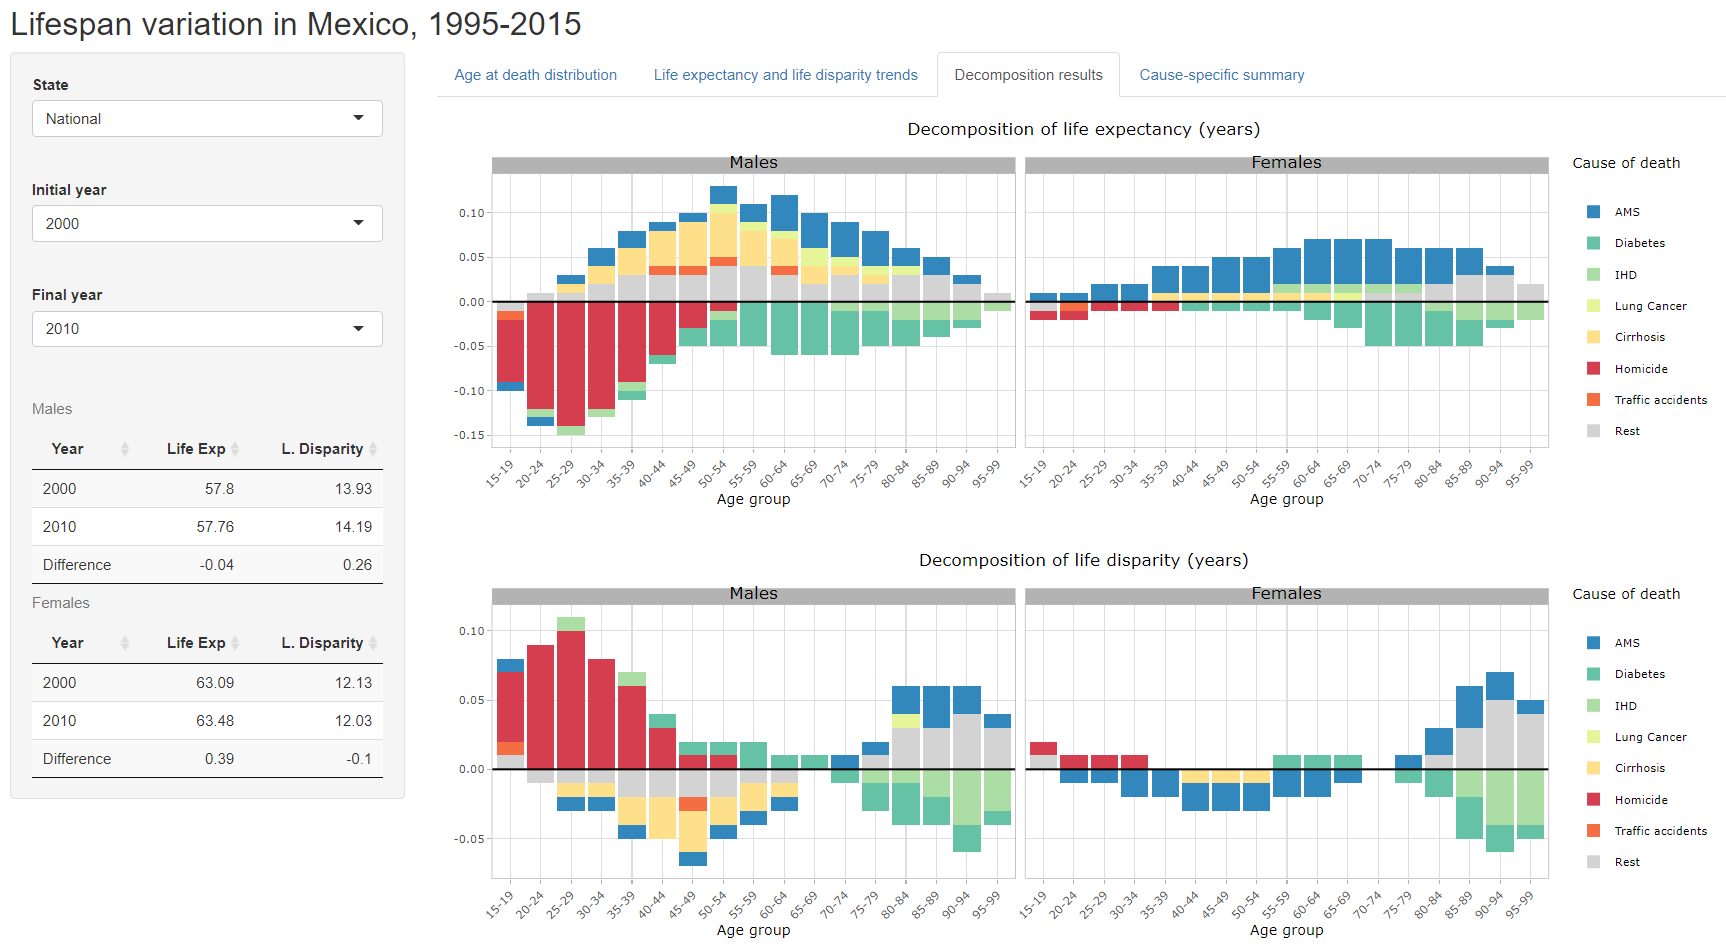
\includegraphics[scale=0.23]{Figures/Shinnyapp_fig} \\   

 

\end{center}
 
 

\end{frame}



\end{document}
	

